\section*{01/11}
\begin{center}
\underline{Конечные элементы более высокого порядка}

\underline{Одномерные квадратичные и кубические функции}
\end{center}
\[
K_x \frac{\partial^2 T}{\partial x^2} + f = 0
\]
\[
\varphi = \alpha_1 + \alpha_2x, \ \dim L = 1, n = 2 \text{ -- симплекс элементы.}
\]

Комплекс элементы -- количество узлов n > 2.  

\begin{center}
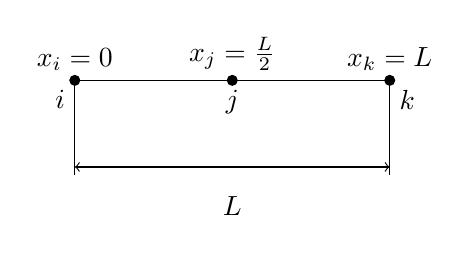
\begin{tikzpicture}[scale=2]
\draw (-1,0) -- (1,0);
\fill (-1,0) circle (1pt) node[below left]{$i$} node[above]{$x_i = 0$};
\fill (0,0) circle (1pt) node[below]{$j$} node[above]{$x_j = \frac{L}{2}$};
\fill (1,0) circle (1pt) node[below right]{$k$} node[above]{$x_k = L$};
\draw (-1,0) -- (-1, -0.6);
\draw (1,0) -- (1, -0.6);
\draw[<->] (-1, -0.55) -- (1, -0.55);
\node at (0, -0.8) {$L$};
\end{tikzpicture}
\end{center}

$\varphi = \alpha_1 + \alpha_2x + \alpha_3x^2 = N \Phi$

В общем виде: $\varphi = \alpha_1 + \alpha_2x + \cdots + \alpha_nx^{n-1}$
\[
\begin{cases}
\Phi_i = \alpha_1 + \alpha_2x_i + \alpha_2x^{2}_i \\
\Phi_j = \alpha_1 + \alpha_2x_j + \alpha_2x^{2}_j \\
\Phi_k = \alpha_1 + \alpha_2x_k + \alpha_2x^{2}_k \\
\end{cases}
\rightarrow \alpha_1, \alpha_2, \alpha_3
\]
\[
\alpha_1 = \Phi_i, \ \alpha_2 = \frac{-3\Phi_i + 4\Phi_j -\Phi_k}{L}, \ \alpha_3 = \frac{2(\Phi_i-2\Phi_j+\Phi_k)}{L^2}
\]
\[
\varphi = \alpha_1 + \alpha_2x + \alpha_3x^2 = 
\]
\[
 = \Phi_i   \underbrace{\left(1 - \frac{3x}{L} + \frac{2x^2}{L^2} \right) }_{N_i}   + \Phi_j \underbrace{\left(\frac{4x}{L} - \frac{4x^2}{L^2} \right)}_{N_j} + \Phi_k \underbrace{\left(-\frac{x}{L} + \frac{2x^2}{L^2} \right)}_{N_k} = 
\]
\[
 = N_i \Phi_i + N_j \Phi_j + N_k \Phi_k = [N]\{\Phi\}
\]
\[
N_i = 1 - \frac{3x}{L} + \frac{2x^2}{L^2}, \ N_j = \frac{4x}{L} - \frac{4x^2}{L^2}, \ N_k = -\frac{x}{L} + \frac{2x^2}{L^2}
\]

Этот же результат можно получить без использования системы уравнений. Зададим в узлах пробные функции $f_{\alpha},\ \alpha \in \{i, j, k\}$, такие, что $f_{\alpha}(x_{\alpha}) = 0$:

\begin{center}
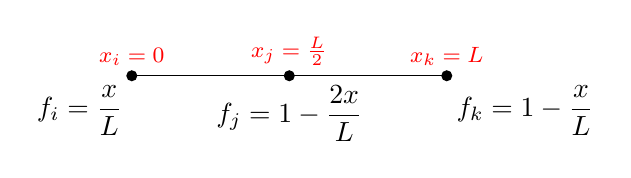
\begin{tikzpicture}[scale=2]
\draw (-1,0) -- (1,0);
\fill (-1,0) circle (1pt) node[below left]{$\displaystyle f_i = \frac{x}{L}$} node[above][red]{\footnotesize$x_i = 0$};
\fill (0,0) circle (1pt) node[below]{$\displaystyle f_j = 1-\frac{2x}{L}$} node[above][red]{\footnotesize$x_j = \frac{L}{2}$};
\fill (1,0) circle (1pt) node[below right]{$\displaystyle f_k = 1-\frac{x}{L}$} node[above][red]{\footnotesize$x_k = L$};
\end{tikzpicture}
\end{center}

Формулы для нахождения функций форм: 
\[
N_i = \frac{f_jf_k}{f_jf_k|_{x = x_i=0}}, \ N_j = \frac{f_if_k}{f_if_k|_{x = x_j=\frac{L}{2}}}, \ N_k = \frac{f_if_j}{f_if_j|_{x = x_k = L}}
\]
\[
N_i = \left(1 - \frac{2x}{L}\right)\cdot \left( 1 - \frac{x}{L} \right), \ N_j = \frac{4x}{L} \cdot \left( 1 - \frac{x}{L}\right), \ N_k = -\frac{x}{L}\cdot \left(1 - \frac{2x}{L}\right)
\]

Аналогично можно найти функции формы для конечных элементов более высокого порядка:
\[\varphi = \alpha_1 + \alpha_2x + \alpha_3x^2 + \alpha_4x^3 = N_i\Phi_i,\ i = 1,\dots, 4\]
\begin{center}
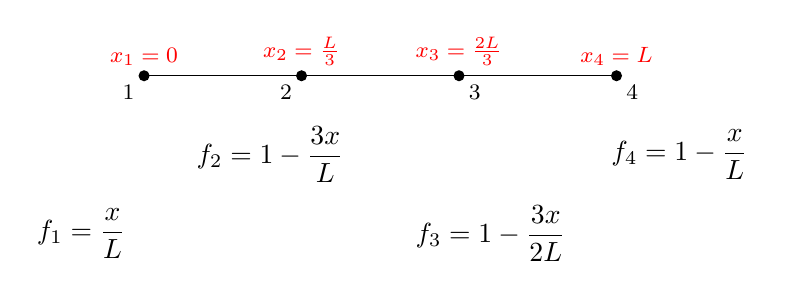
\begin{tikzpicture}[scale=2]
\draw (-1,0) -- (2,0);
\fill (-1,0) circle (1pt) node[below left]{\footnotesize1} node[above][red]{\footnotesize$x_1 = 0$};
\fill (0,0) circle (1pt) node[below left]{\footnotesize2} node[above][red]{\footnotesize$x_2 = \frac{L}{3}$};
\fill (1,0) circle (1pt) node[below right]{\footnotesize3} node[above][red]{\footnotesize$x_3 =  \frac{2L}{3}$};
\fill (2,0) circle (1pt) node[below right]{\footnotesize4} node[above][red]{\footnotesize$x_4 = L$};
\node at (-1.4,-1) {$\displaystyle f_1 = \frac{x}{L}$};
\node at (-0.2,-0.5) {$\displaystyle f_2 = 1 - \frac{3x}{L}$};
\node at (1.2,-1) {$\displaystyle f_3 = 1 - \frac{3x}{2L}$};
\node at (2.4,-0.5) {$\displaystyle f_4 = 1 - \frac{x}{L}$};
\end{tikzpicture}
\end{center}

\begin{center}
\underline{Постановка задачи}
\end{center}
\[K^{(e)} q = P^{(e)}\]
\[K^{(e)} = \int \limits_V B^T D B dV + \int \limits_S \alpha_g N^T N dS\]
\[P^{(e)} = \int \limits_V f N^T dV - \int \limits_S q N^T dS + \int \limits_S \alpha_g T_g N^T dS\]
\[dV = Sdx,\ \ dS = Pdx,\ \text{где } P \text{ -- периметр}\]
\[B = \frac{d[N]}{dx} = \left[ \frac{dN_i}{dx},\ \  \frac{dN_j}{dx},\ \  \frac{dN_k}{dx}\right] = \left[ -\frac{3}{L} + \frac{4x}{L^2},\ \  \frac{4}{L} - \frac{8x}{L^2},\ \  -\frac{1}{L} + \frac{4x}{L^2}\right]\]
\[D = k_x, \text{ так как задача одномерная}\]
Получаем:
\[\int \limits_V B^T D B dV = S k_x \cdot \int \limits_0^L  B^T B dx =\]
\[= Sk_x \cdot \int \limits_0^L
\begin{bmatrix}
\left(-\frac{3}{L} + \frac{4x}{L^2} \right)^2 & \left(-\frac{3}{L} + \frac{4x}{L^2} \right)\left(\frac{4}{L} - \frac{8x}{L^2} \right) & \left(-\frac{3}{L} + \frac{4x}{L^2} \right)\left(-\frac{1}{L} + \frac{4x}{L^2} \right) \\
\left(-\frac{3}{L} + \frac{4x}{L^2} \right)\left(\frac{4}{L} - \frac{8x}{L^2} \right) & \left(\frac{4}{L} - \frac{8x}{L^2} \right)^2 & \left(\frac{4}{L} - \frac{8x}{L^2} \right)\left(-\frac{1}{L} + \frac{4x}{L^2} \right)\\
\left(-\frac{3}{L} + \frac{4x}{L^2} \right)\left(-\frac{1}{L} + \frac{4x}{L^2} \right)& \left(\frac{4}{L} - \frac{8x}{L^2} \right)\left(-\frac{1}{L} + \frac{4x}{L^2} \right) & \left(-\frac{1}{L} + \frac{4x}{L^2} \right)^2
\end{bmatrix} dx =\]
\[= \frac{Sk_x}{6L} \cdot 
\begin{bmatrix}
14 & -16 & 2\\
-16 & 32 & -16\\
2 & -16 & 14
\end{bmatrix}\]

Рассмотрим следующий интеграл:
\[\int \limits_S \alpha_g N^T N dS = P \alpha_g \cdot \int \limits_0^L N^T N dx = P \alpha_g
\cdot \int \limits_0^L \begin{bmatrix}
N_i^2 & N_iN_j & N_iN_k \\
N_iN_j & N_j^2 & N_jN_k \\
N_iN_k & N_jN_k & N_k^2 \\
\end{bmatrix} dx = \]
\[= \frac{\alpha_g P L}{30} \cdot \begin{bmatrix}
4 & 2 & -1 \\
2 & 16 & 2 \\
-1 & 2 & 4 \\
\end{bmatrix}\]

\begin{center}
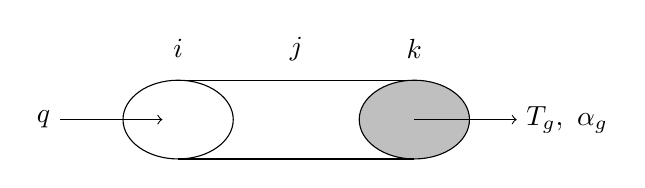
\begin{tikzpicture}
    \fill[gray!50] (2,0) circle (0.7 and 0.5); 
    \draw (-1,0) ellipse (0.7 and 0.5); 
    \draw (2,0) ellipse (0.7 and 0.5); 

    \draw (-1,0.5) -- (2,0.5); 
    \draw (-1,-0.5) -- (2,-0.5); 
    
    \node at (-1, 0.9) {$i$};
    \node at (0.5, 0.9) {$j$};
    \node at (2, 0.9) {$k$};
    
    \draw[<-] (-1.2,0) -- (-2.5,0) node[left] {$q$};
    \draw[->] (2,0) -- (3.3,0) node[right] {$T_g,\ \alpha_g$};
\end{tikzpicture}
\end{center}

Для узла $k$:
\[\alpha_g \int \limits_S N^T N dS = \alpha_g S_k 
\cdot \begin{bmatrix}
0 & 0 & 0 \\
0 & 0 & 0 \\
0 & 0 & 1 \\
\end{bmatrix},\]

где $S_k$ -- площадь сечения для $k$-ого узла.

Для всей боковой поверхности:
\[\alpha_g T_g \int \limits_S N^T dS = \alpha_g T_g P \cdot \int \limits_0^L 
\begin{bmatrix}
N_i \\
N_j \\
N_k \\
\end{bmatrix} dx = 
\frac{\alpha_g T_g P L}{6}
\begin{bmatrix}
1 \\
4 \\
1 \\
\end{bmatrix} \]

Для узла $k$:
\[\alpha_g T_g \int \limits_S N^T dS = \alpha_g T_g S_k 
\begin{bmatrix}
0 \\
0 \\
1 \\
\end{bmatrix} 
\]

Для узла $i$:
\[
\int \limits_S q N^T dS = qS
\begin{bmatrix}
1 \\
0 \\
0 \\
\end{bmatrix} 
\]
\[
\int \limits_V f \cdot N^T dV = S \cdot f \int \limits_0^L N^T dx = \frac{SfL}{6} \cdot
\begin{bmatrix}
1 \\
4 \\
1 \\
\end{bmatrix}
\]

\begin{center}
\underline{Естественная система координат}
\end{center}

\begin{center}
\begin{tikzpicture}
\draw[->] (0,0) -- (5,0) node[below right] {$x$};
\node at (0, -0.4) {0};
\node at (2, -0.8) {$\displaystyle \frac{L}{2}$};
\node at (4, -0.4) {$L$};
\draw (0, 0.1) -- (0, -0.1);
\draw (2, 0.1) -- (2, -0.1);
\draw (4, 0.1) -- (4, -0.1);

\draw[->] (0,-3) -- (5,-3) node[below right] {$\xi$};
\node at (0, -3.4) {-1};
\node at (2, -3.4) {0};
\node at (4, -3.4) {1};
\node[red] at (0, -2.6) {\footnotesize $f_i = 1 + \xi$};
\node[red] at (2, -2.6) {\footnotesize$f_j = \xi$};
\node[red] at (4, -2.6) {\footnotesize$f_k = 1 - \xi$};
\draw (0, -2.9) -- (0, -3.1);
\draw (2, -2.9) -- (2, -3.1);
\draw (4, -2.9) -- (4, -3.1);
\end{tikzpicture}
\end{center}
\[-1 \leq \xi \leq 1,\ x = f(\xi) \Leftrightarrow \xi = \varphi (x)\]
\[\begin{cases}
N_i =\displaystyle \xi (1 - \xi) \cdot \frac{-1}{2} = -\frac{\xi (1 - \xi)}{2},\\
N_j = (1 - \xi)(1 + \xi),\\
N_k =\displaystyle \frac{\xi(1 + \xi)}{2}
\end{cases}\]
\[\varphi = N_i \Phi_i + N_j \Phi_j+ N_k\Phi_k\]
\[x = N_i x_i + N_j x_j+ N_k x_k  \rightarrow x = f(\xi)\]
\[B = \frac{d [N]}{dx};\ \frac{dN_{\beta}}{d\xi} = \frac{dN_{\beta}}{dx} \underbrace{\frac{dx}{d\xi}}_{J},\ J^{-1} =  \frac{1}{\frac{dx}{d\xi}},\ \beta = i, j, k\]
\[\frac{dN_{\beta}}{dx} = J^{-1} \frac{dN_{\beta}}{d\xi}\]
\[J = \frac{dx}{d\xi} = \frac{dN_{i}}{d\xi} x_i + \frac{dN_{j}}{d\xi} x_j + \frac{dN_{k}}{d\xi} x_k \neq \text{const}\]

\begin{center}
\begin{tabular}{cc}
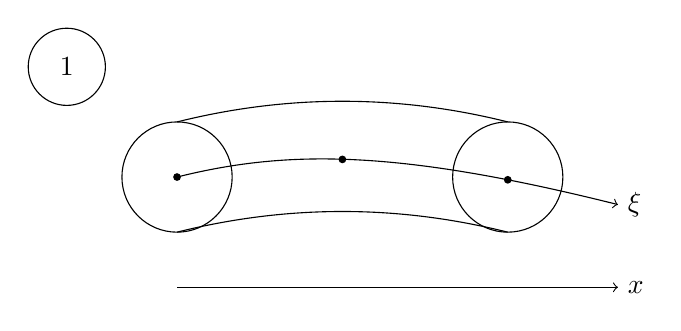
\begin{tikzpicture}[scale=0.7]
    \draw (-2, 2) circle (0.7cm);
    \node at (-2, 2) {1};
    \draw (0,0) circle (1cm);
    \draw (6,0) circle (1cm);
    
    \fill (0,0) circle(2pt);
    \fill (3,0.32) circle(2pt);
    \fill (6,-0.05) circle(2pt);
    
    \draw(0,1) .. controls (2,1.5) and (4, 1.5) .. (6,1); 
    \draw(0,-1) .. controls (2,-0.5) and (4, -0.5) .. (6,-1); 
    \draw[->] (0, 0) .. controls (2, 0.5) and (4, 0.5) .. (8,-0.5) node[right] {$\xi$}; 
    
    \draw[->] (0,-2) -- (8,-2) node[right] {$x$};
\end{tikzpicture}
& 
$\begin{cases}
x = N_i x_i + N_j x_j+ N_k x_k\\
\varphi = N_i \Phi_i + N_j \Phi_j+ N_k\Phi_k
\end{cases}$ \\
Криволинейный стержень & \\
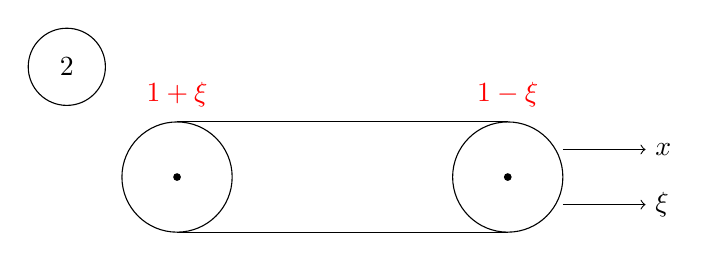
\begin{tikzpicture}[scale=0.7]
    \draw (-2, 2) circle (0.7cm);
    \node at (-2, 2) {2};
    \draw (0,0) circle (1cm);
    \draw (6,0) circle (1cm);
    
    \draw (0,1) -- (6,1);
    \draw (0,-1) -- (6,-1);
    
    \fill (0,0) circle(2pt);
    \fill (6,0) circle(2pt);
    
    \node[red] at (0, 1.5) {$1 + \xi$};
    \node[red] at (6, 1.5) {$1 - \xi$};
    
    \draw[->] (7,0.5) -- (8.5, 0.5) node[right] {$x$};
    \draw[->] (7,-0.5) -- (8.5, -0.5) node[right] {$\xi$};
    
\end{tikzpicture}
&
$\begin{cases}
x = \tilde{N_i} x_i + \tilde{N_k} x_k\\
\tilde{N_i} = \displaystyle \frac{1}{2} (1 - \xi),\ \tilde{N_k} = \displaystyle \frac{1}{2} (1 + \xi)\\
\varphi = N_i \Phi_i + N_j \Phi_j+ N_k\Phi_k
\end{cases}$ \\
Линейный стержень  & (если в задании нужно вычислить \\
(задаем через две точки)  & что-то в середине, то используем \\
& квадратичные функции формы) \\

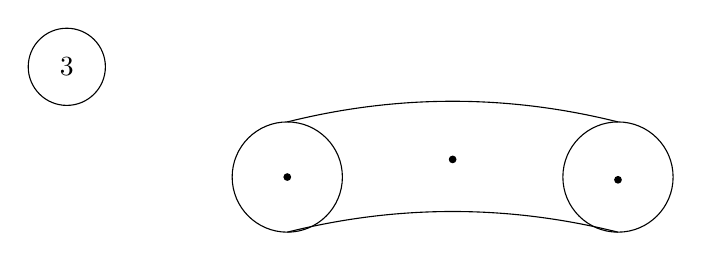
\begin{tikzpicture}[scale=0.7]
    \draw (-4, 2) circle (0.7cm);
    \node at (-4, 2) {3};
    \draw (0,0) circle (1cm);
    \draw (6,0) circle (1cm);
    
    \fill (0,0) circle(2pt);
    \fill (3,0.32) circle(2pt);
    \fill (6,-0.05) circle(2pt);
    
    \draw(0,1) .. controls (2,1.5) and (4, 1.5) .. (6,1); 
    \draw(0,-1) .. controls (2,-0.5) and (4, -0.5) .. (6,-1); 
    \end{tikzpicture}
& 
$\begin{cases}
x = N_i x_i + N_j x_j+ N_k x_k\\
\varphi = \tilde{N_i} \Phi_i + \tilde{N_k}\Phi_k
\end{cases}$ \\
Криволинейный элемент & (достаточно рассмотреть только \\
& на концах элемента) \\
\end{tabular}
\end{center}

Пусть $A$ -- количество узлов для задания формы элемента ($x = f(\xi)$), $B$ -- количество узлов для задания интерполяционного полинома ($\varphi$).
\begin{enumerate}
\item Если $A = B$, такой конечный элемент называется \textit{изопараметрический}.
\item Если $A < B$, такой конечный элемент называется \textit{субпараметрический}.
\item Если $A > B$, такой конечный элемент называется \textit{суперпараметрический}.
\end{enumerate}